\clearpage
\section{Systematic uncertainties}
\label{tW_systematic}

This analysis depends on both the normalization and shape of the background and signal expectations.
We consider the following sources of systematic uncertainties which affect the shape and normalization of the templates used in the statistical evaluation:




$\bullet$ \textit{\textbf{\ttbar~ and $tW$ modeling uncertainty:}} there are various input for generating and simulating \ttbar~ and $tW$ processes. In Table \ref{mc-samples-sys}, related samples used for studying the effect of the modeling uncertainties are sorted.
The \ttbar~ and $tW$ modeling uncertainty sources are

\begin{itemize}
  \item {\textit{\textbf{QCD scale uncertainty:}} This uncertainty is estimated by varying the renormalization and the factorization scales, used during the MC generation of the sample, independently by a factor 0.5, 1 or 2. Unphysical cases, where one scale fluctuate up while the other fluctuate down, are not considered. An envelope is built from all the 6 possible variations by taking in each bin of the distribution the maximum (minimum) variation and is used as an estimate of the QCD scale uncertainties for \ttbar~ sample. For $tW$, independent samples are used (see Table \ref{mc-samples-sys}).}
%  \item {\textit{\textbf{Parton Distribution Functions uncertainty:}} The magnitude of the uncertainties related to the parton distribution functions and the variation of the strong coupling constant for each simulated signal processes is obtained using the replicas of the NNPDF 3.0 set. $tW$ sample is generated by powheg v1 generator and PDF weights are not available in the samples. We will use MadgraphAmc@NLO sample to evaluate PDF uncertainty on $tW$ (***Note this uncertainty for \ttbar~ will be added in next version of the note). }
  \item {\textit{\textbf{Parton Distribution Functions uncertainty:}} The magnitude of the uncertainties related to the parton distribution functions and the variation of the strong coupling constant for each simulated signal processes is obtained using the replicas of the NNPDF 3.0 set (***NOTE no weight for calculating the PDF uncertainty is presented in tW samples. So this uncertainty is not included for tW).}
  \item \textit{\textbf{Top mass:}} The most recent measurement of the top quark mass by CMS yields a total uncertainty of $\pm 0.49$  GeV. We consider a sample with varied top mass at  $m_t=172.5\pm3.0$  GeV and reduce the obtained uncertainty by a factor of 6.
  \item \textit{\textbf{$tW$/\ttbar~ interference:}} At NLO QCD, tW production is expected to interfere with \ttbar~ production \cite{Demartin:2016axk}. Two schemes for defining the tW signal in a way which distinguishes it from \ttbar~ production have been compared in our analysis: 'diagram removal' (DR), in which all
doubly resonant NLO $tW$ diagrams are removed,  and 'diagram subtraction' (DS), where a gauge-invariant subtractive term modifies the NLO tW cross section to locally cancel the contribution from \ttbar~. The difference between the samples simulated using the two approaches is taken as a systematic uncertainty.
  \item \textit{\textbf{ME/PS matching:}} The model parameter $h_{damp}$ in
POWHEG that controls the matching of the matrix elements to the PYTHIA parton showers is varied from its default value of 172.5 GeV
by factors of 0.5 and 2. This source of uncertainty is only considered for \ttbar~.
  \item \textit{\textbf{scale variations of initial state radiation (ISR) and final state radiation FSR: }} From a practical point of view, we vary the renormalization scale for QCD emissions in  FSR and ISR by a factor of 0.5 and 2. The uncertainty for the FSR shower scale variation is reduced by a factor of $\sqrt{2}$ following the TOP PAG recommendations.
  \item \textit{\textbf{Underlying event:}} the default parameters in the CUETP8M2T4 are varied according to their uncertainty and the effect on the unfolding is taken as an estimate of the systematic uncertainty. This source of uncertainty is only considered for \ttbar.
  \item \textit{\textbf{Color reconnection:}} we vary the color reconnection model with respect to the default using alternatives including the resonant decay products in possible reconnections to the UE. The default simulation (MPI-based color reconnection) has this effect excluded. We examine three alternative models for CR: the so-called gluon move, early resonance decay and the QCD-inspired models. The envelope of the differences is considered as a systematic uncertainty. This source of uncertainty is only considered for \ttbar.
\end{itemize}

\begin{table}[h]
\centering
\small
\smallskip\noindent
\resizebox{\linewidth}{!}{%
\begin{tabular}{l|l}
\hline
Sample                                                                       &Events\\ \hline
\hline
Nominal:TTTo2L2Nu\_TuneCUETP8M2\_ttHtranche3\_13TeV-powheg                           & 64910035        \\
Nominal:ST\_tW\_top\_5f\_NoFullyHadronicDecays\_13TeV-powheg\_TuneCUETP8M1           & 8609398         \\
Nominal:ST\_tW\_antitop\_5f\_NoFullyHadronicDecays\_13TeV-powheg\_TuneCUETP8M1       & 8681265         \\
\hline
ST\_tW\_top\_5f\_DS\_NoFullyHadronicDecays\_13TeV-powheg-pythia8             &3192538\\
ST\_tW\_antitop\_5f\_DS\_NoFullyHadronicDecays\_13TeV-powheg-pythia8         &3098002\\
ST\_tW\_top\_5f\_MEscaleup\_NoFullyHadronicDecays\_13TeV-powheg              &3188665\\
ST\_tW\_antitop\_5f\_MEscaleup\_NoFullyHadronicDecays\_13TeV-powheg          &1606961\\
ST\_tW\_top\_MEscaledown\_5f\_NoFullyHadronicDecays\_13TeV-powheg            &3051991\\
ST\_tW\_antitop\_MEscaledown\_5f\_NoFullyHadronicDecays\_13TeV-powheg        &1575142\\
ST\_tW\_top\_5f\_mtop1695\_NoFullyHadronicDecays\_13TeV-powheg-pythia8       &3178900\\
ST\_tW\_antitop\_5f\_mtop1695\_NoFullyHadronicDecays\_13TeV-powheg-pythia8   &2968744\\
ST\_tW\_top\_5f\_mtop1755\_NoFullyHadronicDecays\_13TeV-powheg-pythia8       &2938402\\
ST\_tW\_antitop\_5f\_mtop1755\_NoFullyHadronicDecays\_13TeV-powheg-pythia8   &3194626\\
ST\_tW\_top\_5f\_isrup\_NoFullyHadronicDecays\_13TeV-powheg                  &3110339\\
ST\_tW\_top\_isrdown\_5f\_NoFullyHadronicDecays\_13TeV-powheg                &3181500\\
ST\_tW\_antitop\_5f\_isrup\_NoFullyHadronicDecays\_13TeV-powheg              &3076275\\
ST\_tW\_antitop\_isrdown\_5f\_NoFullyHadronicDecays\_13TeV-powheg            &3101321\\
ST\_tW\_top\_5f\_fsrup\_NoFullyHadronicDecays\_13TeV-powheg                  &3192325\\
ST\_tW\_top\_fsrdown\_5f\_NoFullyHadronicDecays\_13TeV-powheg                &2935595\\
ST\_tW\_antitop\_5f\_fsrup\_NoFullyHadronicDecays\_13TeV-powheg              &3001527\\
ST\_tW\_antitop\_fsrdown\_5f\_NoFullyHadronicDecays\_13TeV-powheg            &3234964\\
\hline
TT\_TuneCUETP8M2T4\_QCDbasedCRTune\_erdON\_13TeV-powheg-pythia8              &57788977\\
TT\_TuneCUETP8M2T4\_erdON\_13TeV-powheg-pythia8                              &58448827\\
TT\_TuneCUETP8M2T4\_GluonMoveCRTune\_13TeV-powheg-pythia8                    &56456001\\
TT\_TuneCUETP8M2T4\_mtop1695\_13TeV-powheg-pythia8                           &58281931\\
TT\_TuneCUETP8M2T4\_mtop1755\_13TeV-powheg-pythia8                           &38909457\\
TT\_TuneCUETP8M2T4\_13TeV-powheg-fsrdown-pythia8                             &57563666\\
TT\_TuneCUETP8M2T4\_13TeV-powheg-fsrup-pythia8                               &58475264\\
TT\_TuneCUETP8M2T4\_13TeV-powheg-isrdown-pythia8                             &58421030\\
TT\_TuneCUETP8M2T4\_13TeV-powheg-isrup-pythia8                               &57577179\\
TT\_hdampDOWN\_TuneCUETP8M2T4\_13TeV-powheg-pythia8                          &55809842\\
TT\_hdampUP\_TuneCUETP8M2T4\_13TeV-powheg-pythia8                            &58320199\\
TT\_TuneCUETP8M2T4down\_13TeV-powheg-pythia8                                 &57721717\\
TT\_TuneCUETP8M2T4up\_13TeV-powheg-pythia8                                   &58144172\\
\hline
\hline
\end{tabular}}
\caption{MC samples used for systematic study}
\label{mc-samples-sys}
\end{table}


 In figures \ref{fig:uncert_TT}-\ref{fig:uncert_TW}, the relative effect of each source of \ttbar~ and $tW$ modeling uncertainties for the MLP output distributions are shown. Relative uncertainties stands for the ratio of MLP for tW (\ttbar) systematic sample to nominal tW (\ttbar) sample. All modeling uncertainties are shape dependent uncertainties.


\begin{figure}[ht]
  \begin{center}
    \begin{tabular}{ccc}
      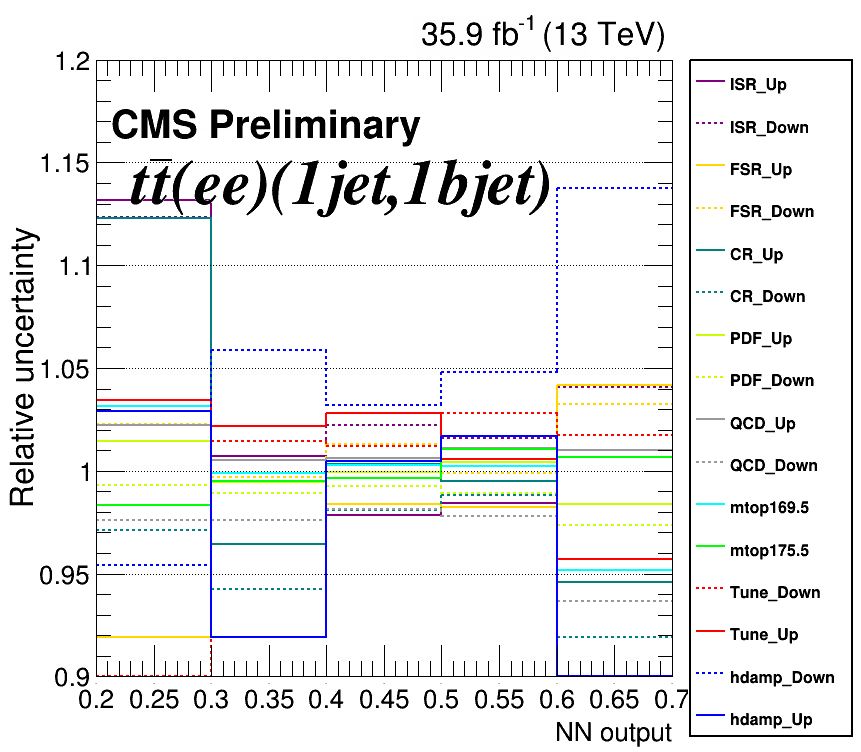
\includegraphics[width=0.4\textwidth]{figures/tW/fig/Step2/uncertainties/ee/TT_Samples_H_MLP_1jet_1bjet_comb.png} &
      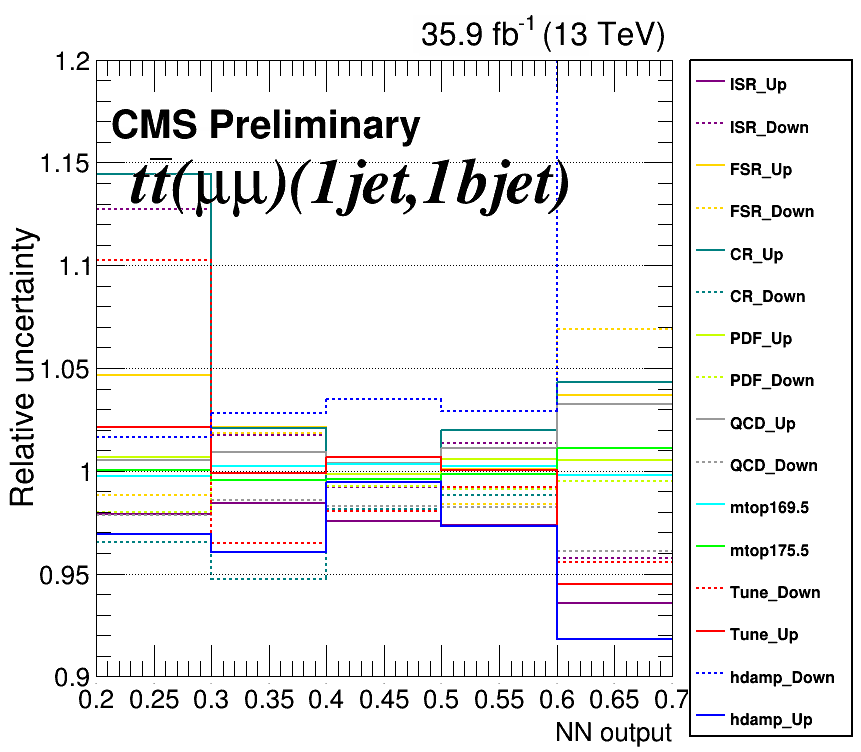
\includegraphics[width=0.4\textwidth]{figures/tW/fig/Step2/uncertainties/mumu/TT_Samples_H_MLP_1jet_1bjet_comb.png}\\
      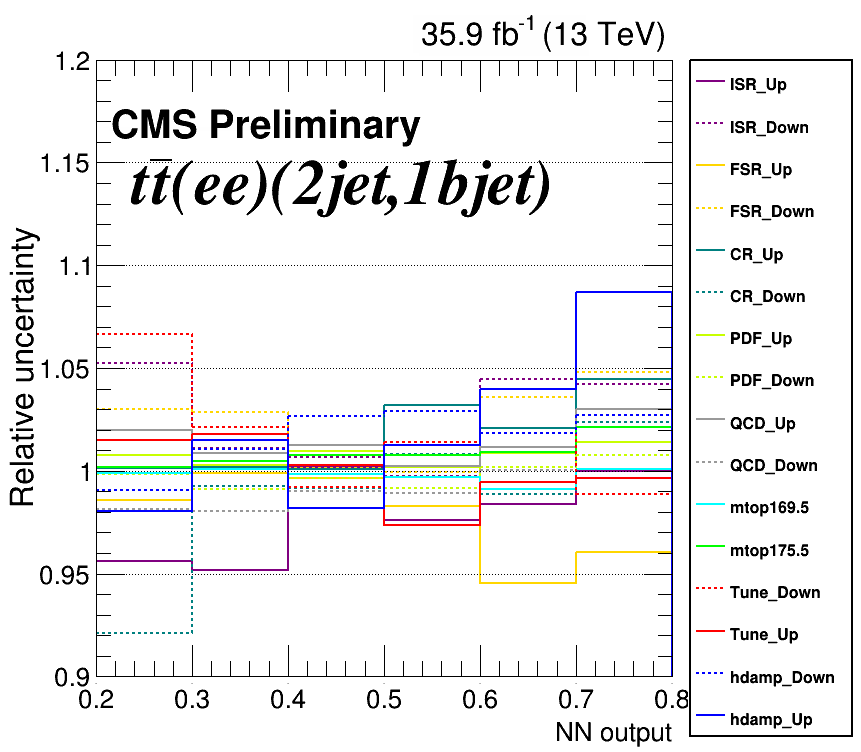
\includegraphics[width=0.4\textwidth]{figures/tW/fig/Step2/uncertainties/ee/TT_Samples_H_MLP_2jet_1bjet_comb.png} &
      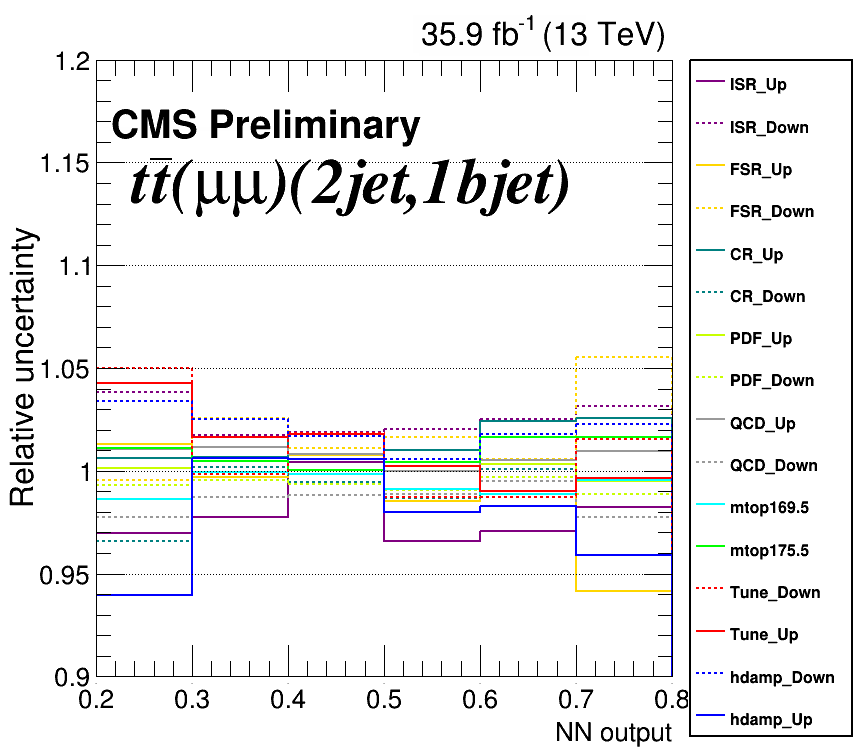
\includegraphics[width=0.4\textwidth]{figures/tW/fig/Step2/uncertainties/mumu/TT_Samples_H_MLP_2jet_1bjet_comb.png}\\
    \end{tabular}
    \caption{The relative effect of the \ttbar~ modeling uncertainties in MLP distribution for different (1jet,1b-jet) region (top row), (2jet,1b-jet) region (bottom row) for $ee$ channel (left column) and $\mu\mu$ channel (right column).
    \label{fig:uncert_TT}}
  \end{center}
\end{figure}

\begin{figure}[ht]
  \begin{center}
    \begin{tabular}{ccc}
      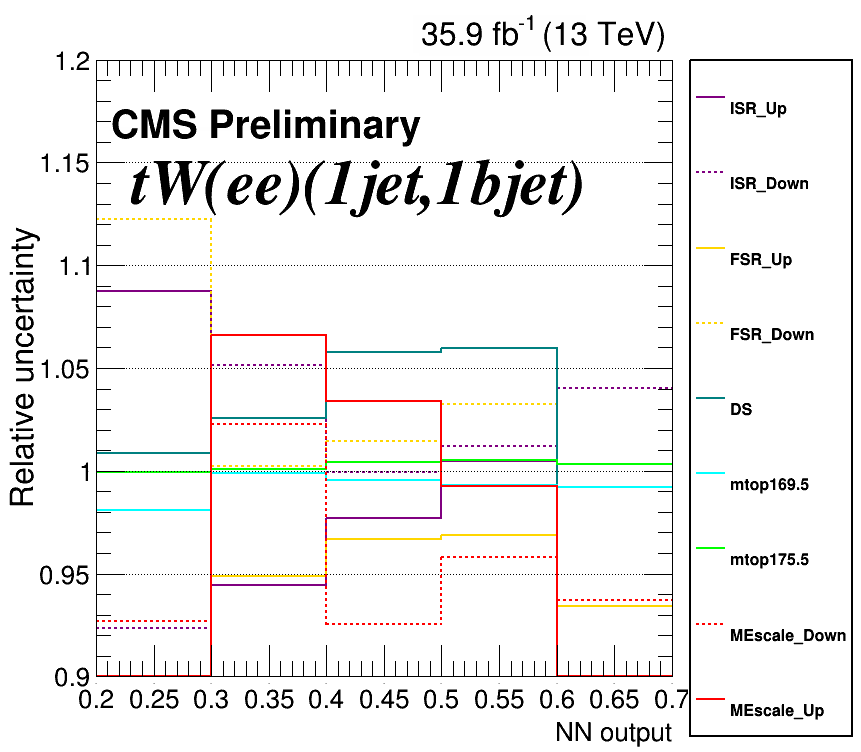
\includegraphics[width=0.4\textwidth]{figures/tW/fig/Step2/uncertainties/ee/TW_Samples_H_MLP_1jet_1bjet_comb.png} &
      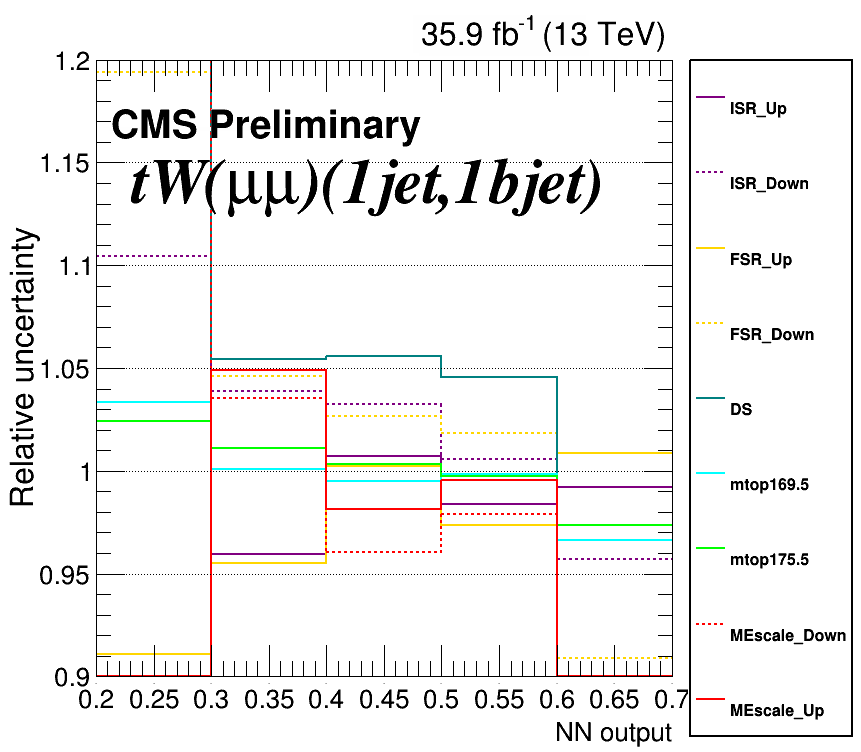
\includegraphics[width=0.4\textwidth]{figures/tW/fig/Step2/uncertainties/mumu/TW_Samples_H_MLP_1jet_1bjet_comb.png}\\
      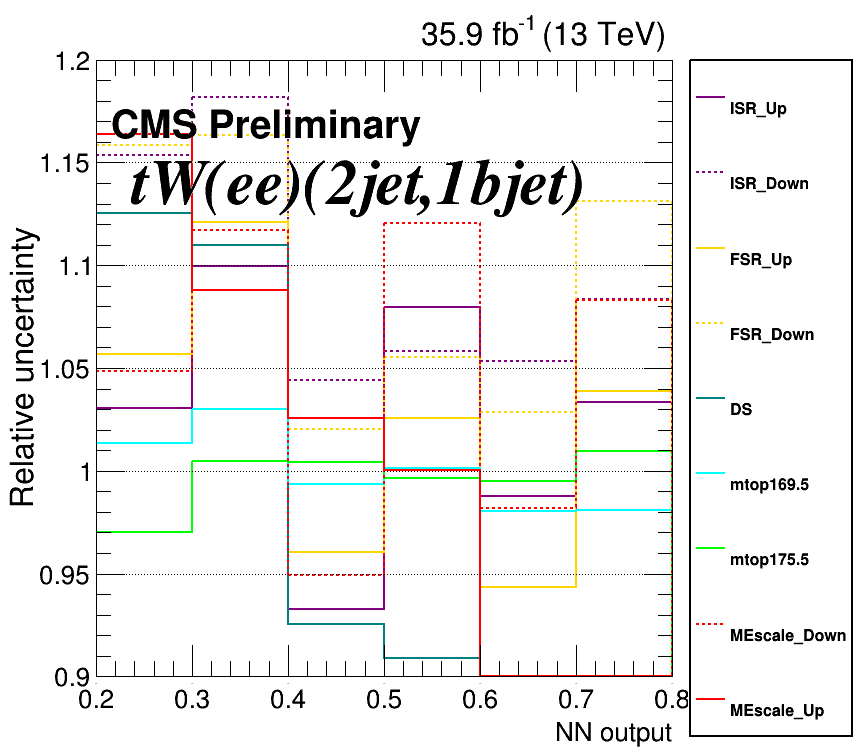
\includegraphics[width=0.4\textwidth]{figures/tW/fig/Step2/uncertainties/ee/TW_Samples_H_MLP_2jet_1bjet_comb.png} &
      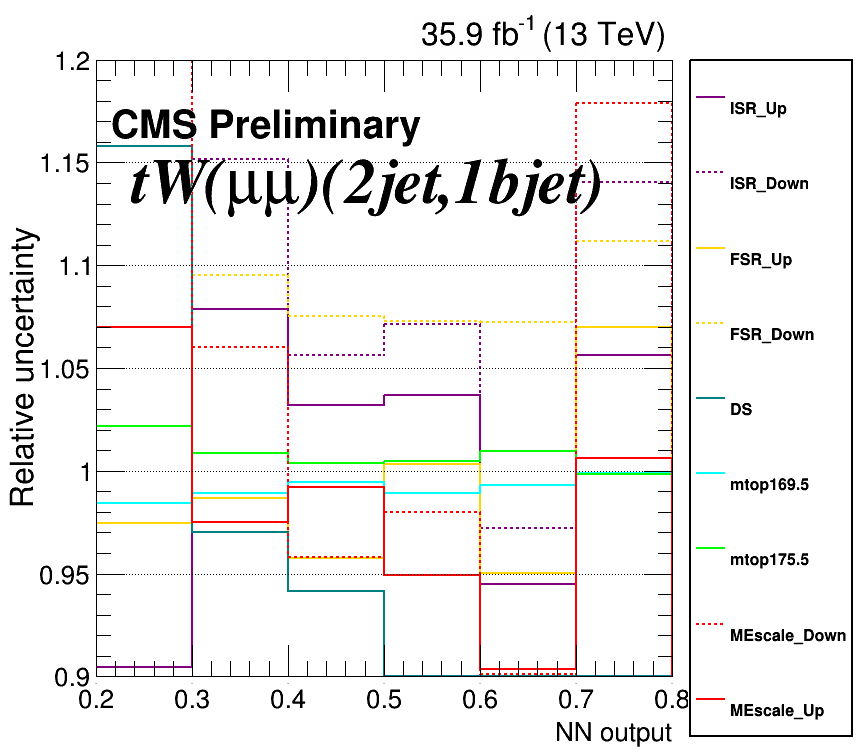
\includegraphics[width=0.4\textwidth]{figures/tW/fig/Step2/uncertainties/mumu/TW_Samples_H_MLP_2jet_1bjet_comb.png}\\
    \end{tabular}
    \caption{The relative effect of the tW modeling uncertainties in MLP distribution for different (1jet,1b-jet)  region (top row), (2jet,1b-jet) region (bottom row) for $ee$ channel (left column) and $\mu\mu$ channel (right column).
    \label{fig:uncert_TW}}
  \end{center}
\end{figure}

\clearpage





$\bullet$ \textit{\textbf{Lepton reconstruction, identification and isolation scale factors:}} Electrons and muons reconstruction, isolation and identification scale factors and uncertainties are provided centrally by related POGs, extracted with a tag-and-probe analysis on Z to ll events.

$\bullet$ \textit{\textbf{Jet energy scale and resolution:}} uncertainties in the jet energy scale and resolution is provided officially by JET/MET POG in the recommended global tag \cite{GT}.
In order to find the latest jet energy scale uncertainty, '80X\_mcRun2\_asymptotic\_2016\_TrancheIV\_v8' global tag is used.
Variation of jet energy scale and resolution are propagated to MET and MET is corrected due to the changes.

$\bullet$ \textit{\textbf{Unclustered energy  uncertainty:}} uncertainty on unclustered energy is considered which propagated to MET and MET is corrected due to the changes.

$\bullet$ \textit{\textbf{Trigger scale factor:}} uncertainty on the  trigger scale factor are provided in TOP recommended scale factor root files.

$\bullet$  \textit{\textbf{b-tagging}}: The efficiency for b-tagging is determined for the baseline selection and then scaled up and down according to their uncertainties given by the BTV group. The b-quark and c-quark jet efficiencies are varied simultaneously, while the efficiencies for the light quarks are varied independently \cite{btag}.

$\bullet$  \textit{\textbf{Pile-up reweighting}}: The measured minimum-bias cross section ($69.2$ mb) is varied by 4.6\% to produce
different expected pileup distributions for data (up and down).

$\bullet$ \textit{\textbf{Luminosity:}} A systematic uncertainty of 2.5\% is assigned to the integrated luminosity
and is used for background rates \cite{CMS-PAS-LUM-17-001}.

$\bullet$ \textit{\textbf{\ttbar~ normalization:}} uncertainty on \ttbar~ normalization is considered to be  5\% \cite{Khachatryan:2016kzg} for $O_{\phi q}^{(3)}$, $O_{tW}$, $O_{uG}$ and $O_{cG}$ study, 3\% for $O_{G}$ study due to the observed difference between the \ttbar~ kinematic distribution with and without $O_{G}$.

$\bullet$ \textit{\textbf{tW normalization:}} uncertainty on tW normalization is considered to be  10\% for $O_{uG}$, $O_{cG}$ and $O_{G}$ study.

$\bullet$ \textit{\textbf{Non-top background normalization:}} uncertainty on DY normalization in $ee$ and $\mu\mu$ channels (data-driven normalization) is considred to be 30\% in all njet-mtag regions. DY normalization uncertainty is considered to be uncorrelated between various njet-mbtag regions. The uncertainty on other and jet backgrounds are considered to be 50\%.

\medskip
For FCNC signal ($O_{uG}$ and $O_{cG}$) study, additional uncertainties are considered in following.

   $\bullet$ \textit{\textbf{Parton Distribution Functions uncertainty:}} The magnitude of the uncertainties related to the parton distribution functions and the variation of the strong coupling constant for FCNC tW simulated signal processes is obtained using the replicas of the NNPDF 3.0 set. Each event is weighted with respect to the LHE weights provided for each replicas of the NNPDF 3.0 set and final NN distribution is found. One sigma UP/DOWN uncertainty from the distribution of the NN output due to the various PDF set  with respect to  the nominal set is assigned as PDF error.

   $\bullet$ \textit{\textbf{QCD scale uncertainty:}} This uncertainty is estimated by varying the renormalization and the factorization scales for FCNC tW simulated signal, used during the MC generation of the sample by a factor 0.5 and or 2. Each event is weighted with respect to the LHE weights provided for renomalization and factorization scale variation. The largest deviation from the nominal value is taken as QCD scale error.

   $\bullet$ \textit{\textbf{Parton shower Q scale uncertainty:}} The scales of the initial (ISR) and final (FSR) state shower are varied up and down by a factor of two FCNC tW simulated signal samples. MC samples used to estimate the parton shower Q scale uncertainties are sumarrised in Table \ref{sysFCNC}.

\begin{table}[h]
\centering
\begin{tabular}{l}
\hline
sample                                                  \\
\hline
\hline
ST\_tW\_tcgFCNC\_scaledown\_leptonDecays\_Madgraph                \\
ST\_tW\_tcgFCNC\_scaleup\_leptonDecays\_Madgraph                \\
ST\_tW\_tugFCNC\_scaledown\_leptonDecays\_Madgraph               \\
ST\_tW\_tugFCNC\_scaleup\_leptonDecays\_Madgraph                \\
\hline
\end{tabular}
\caption{Systematic samples for FCNC signal study}
\label{sysFCNC}
\end{table}




In Figure \ref{fig:uncert_shape}, the effect of shape dependent uncertainties except \ttbar~ and $tW$ modeling are shown.

The relative effect of the all uncertainties on the total normalization are summarized in tables \ref{tab:ee_all}, and \ref{tab:mumu_all} for $ee$ and $\mu\mu$ channel respectively.

%
%\begin{figure}[ht]
%  \begin{center}
%    \begin{tabular}{ccc}
%      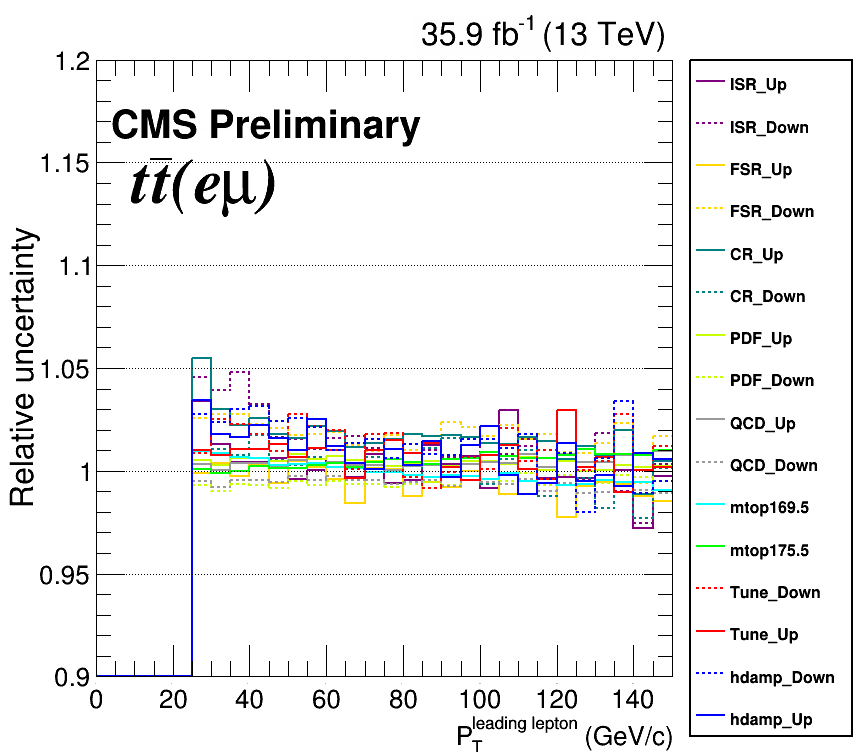
\includegraphics[width=0.32\textwidth]{figures/tW/fig/Step2/emu_modeling/TT_Samples_H_lepton_led_pt.png}&
%      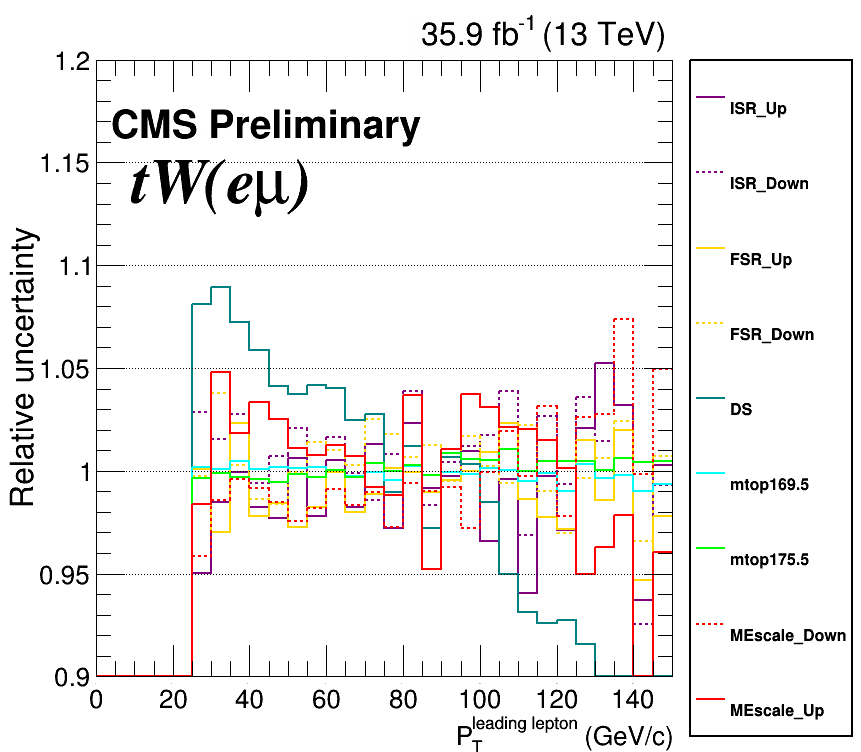
\includegraphics[width=0.32\textwidth]{figures/tW/fig/Step2/emu_modeling/TW_Samples_H_lepton_led_pt.png}\\
%      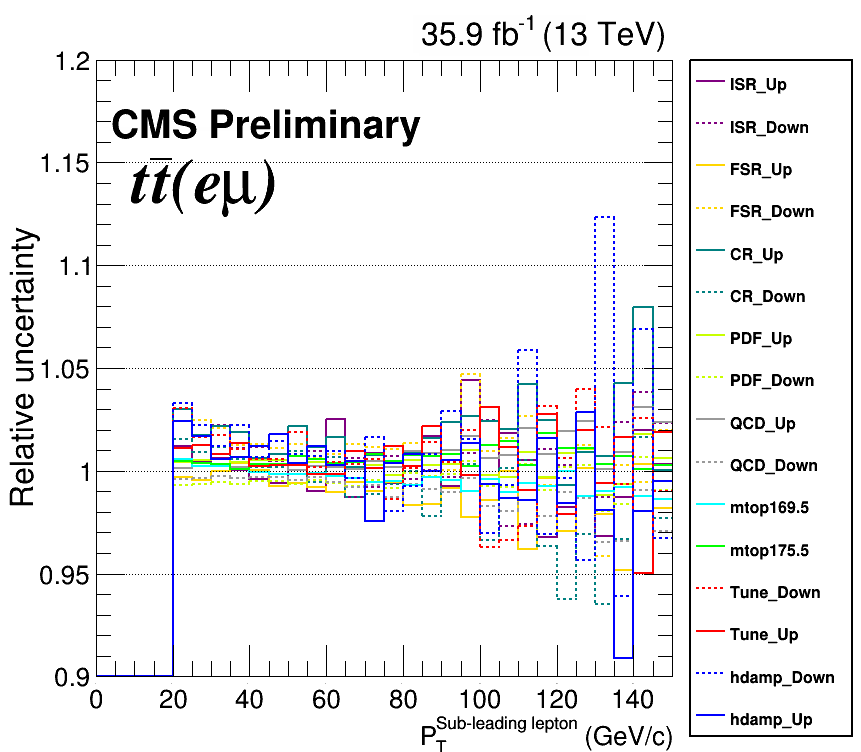
\includegraphics[width=0.32\textwidth]{figures/tW/fig/Step2/emu_modeling/TT_Samples_H_lepton_sub_pt.png}&
%      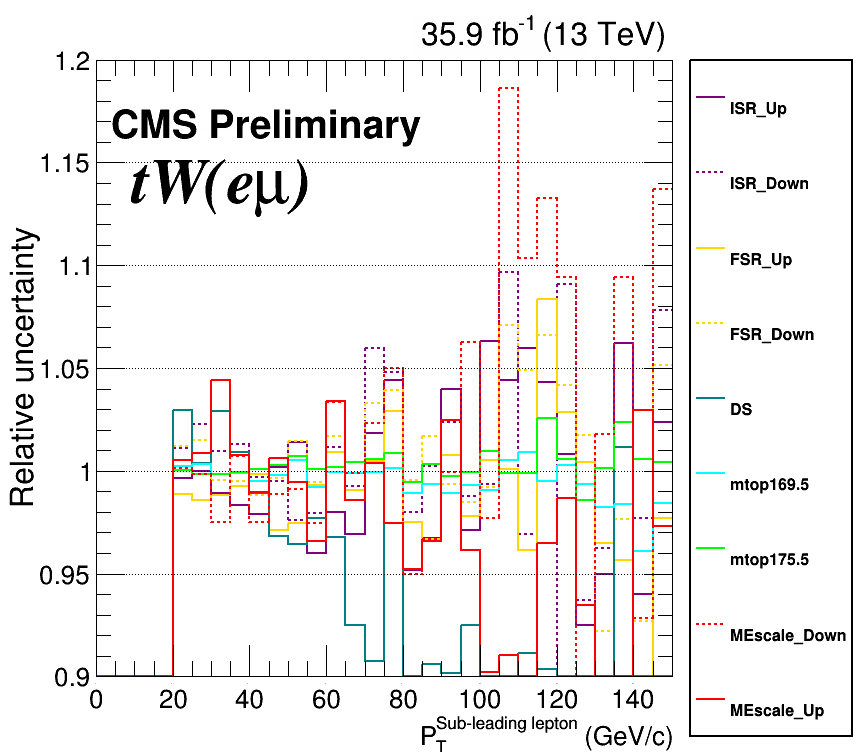
\includegraphics[width=0.32\textwidth]{figures/tW/fig/Step2/emu_modeling/TW_Samples_H_lepton_sub_pt.png}\\
%      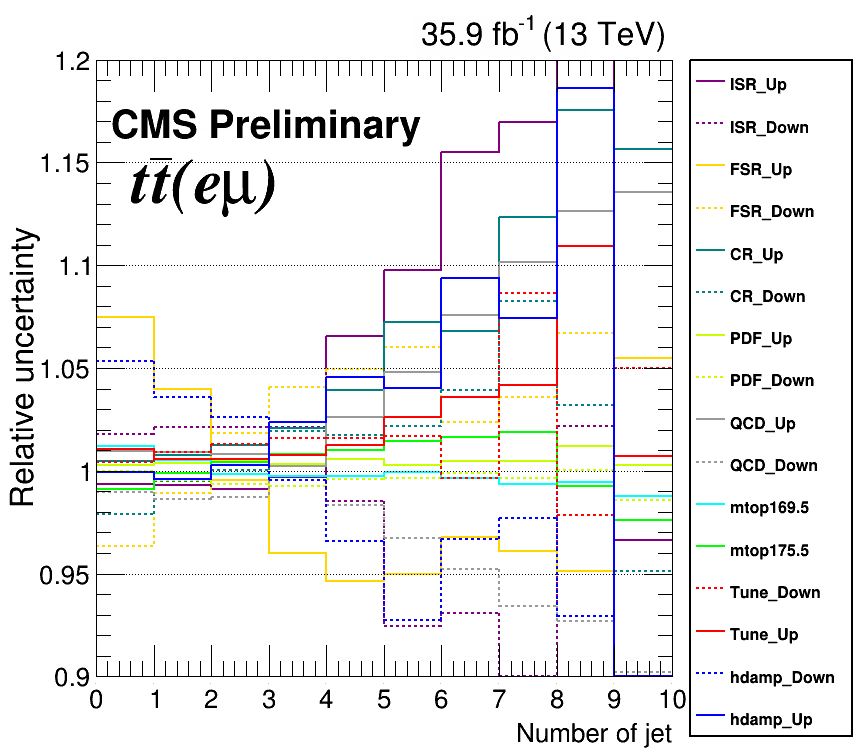
\includegraphics[width=0.32\textwidth]{figures/tW/fig/Step2/emu_modeling/TT_Samples_H_N_loose_jets.png}&
%      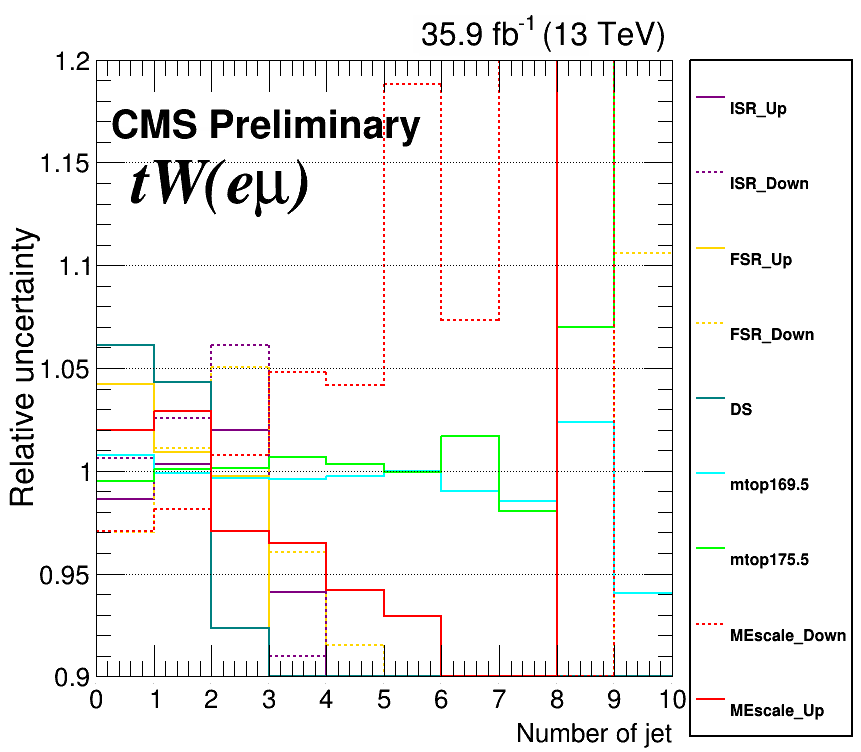
\includegraphics[width=0.32\textwidth]{figures/tW/fig/Step2/emu_modeling/TW_Samples_H_N_loose_jets.png}\\
%      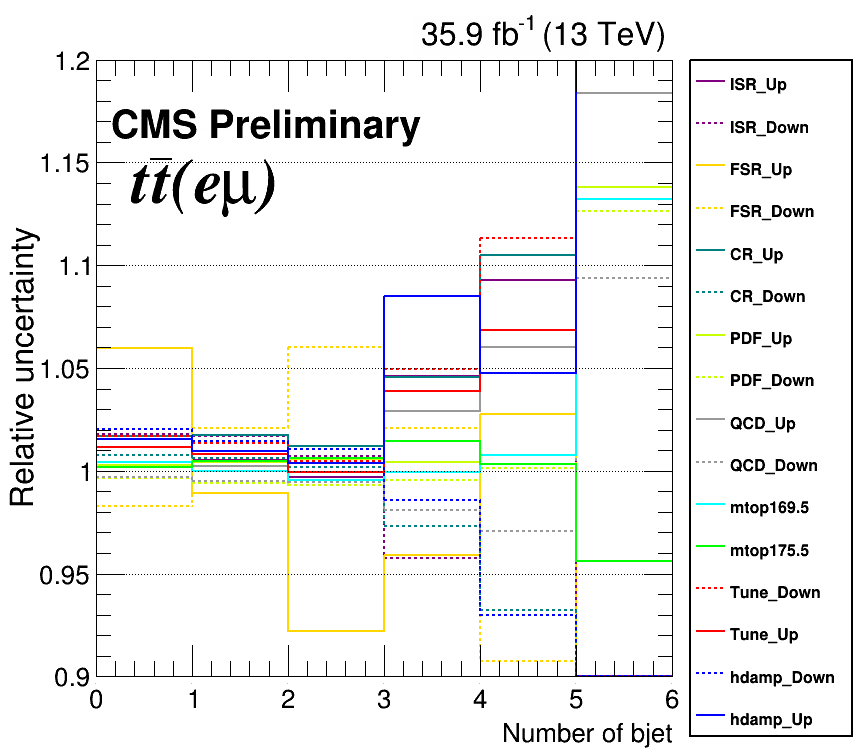
\includegraphics[width=0.32\textwidth]{figures/tW/fig/Step2/emu_modeling/TT_Samples_H_N_b_jets.png}&
%      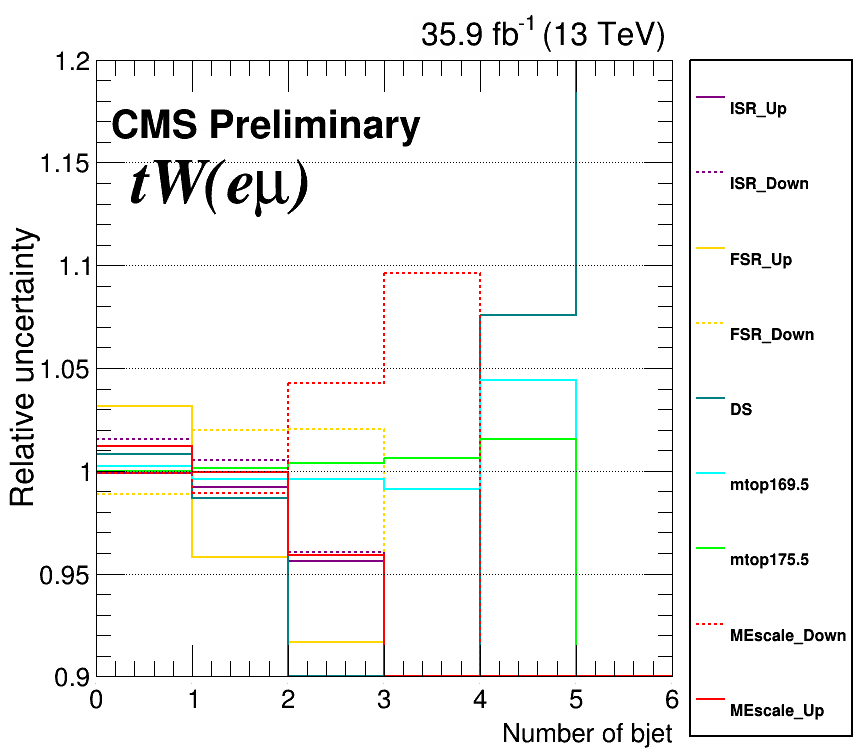
\includegraphics[width=0.32\textwidth]{figures/tW/fig/Step2/emu_modeling/TW_Samples_H_N_b_jets.png}\\
%    \end{tabular}
%    \caption{The distributions of leading lepton Pt (first row), Pt of sub-leading lepton (second row), number of jet (third row) and number of b jet (last row) for $t\bar(t)$ (left) and $tW$ (right) for different models after step 2.
%    \label{fig:modeling}}
%  \end{center}
%\end{figure}
%
%\begin{figure}[ht]
%  \begin{center}
%    \begin{tabular}{ccc}
%      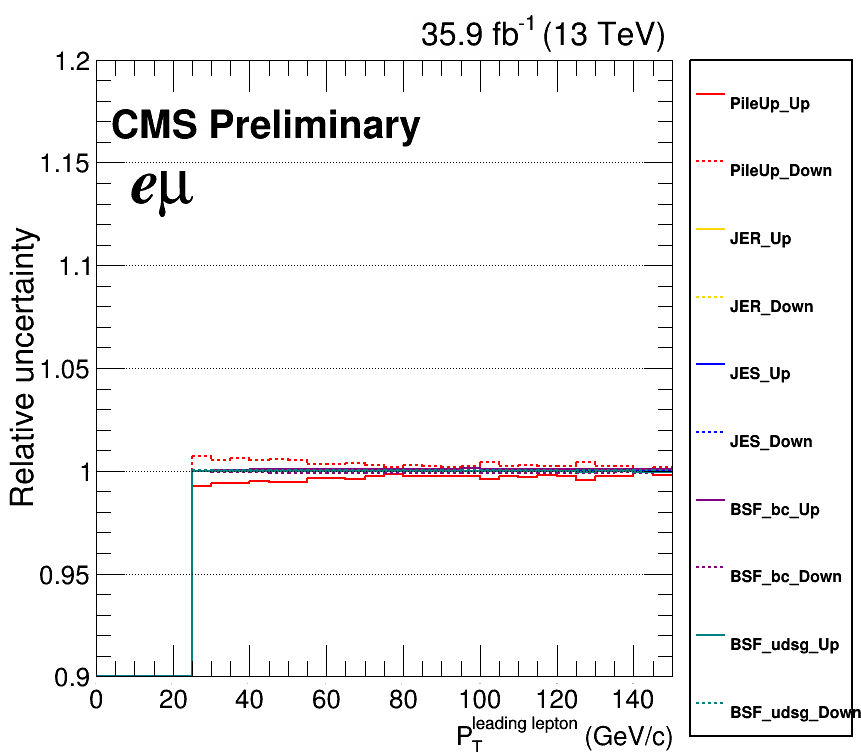
\includegraphics[width=0.32\textwidth]{figures/tW/fig/Step2/emu_shape_uncert/Shape_uncert_H_lepton_led_pt.png}&
%      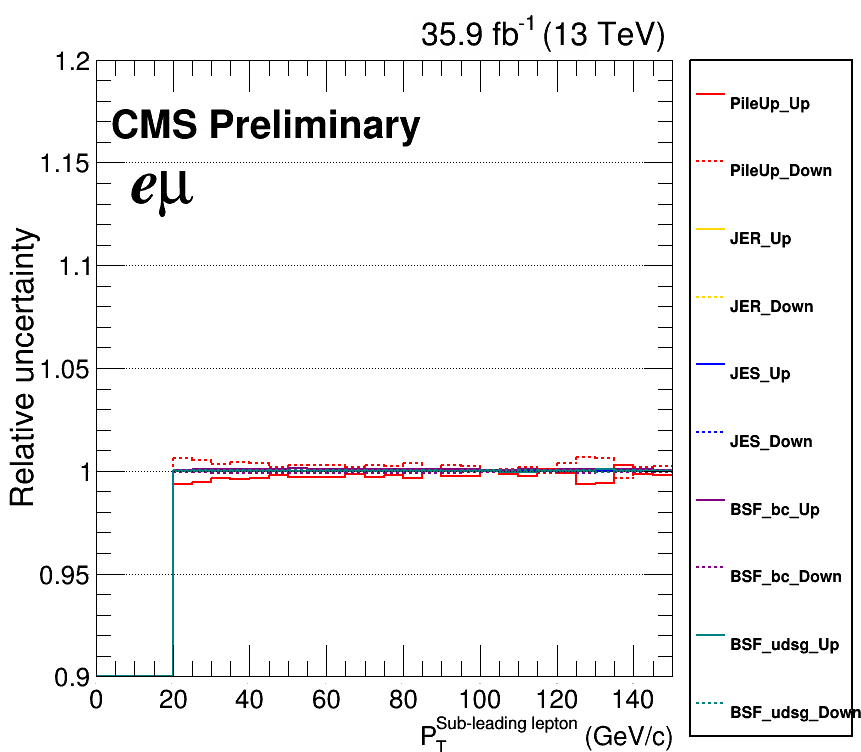
\includegraphics[width=0.32\textwidth]{figures/tW/fig/Step2/emu_shape_uncert/Shape_uncert_H_lepton_sub_pt.png}\\
%      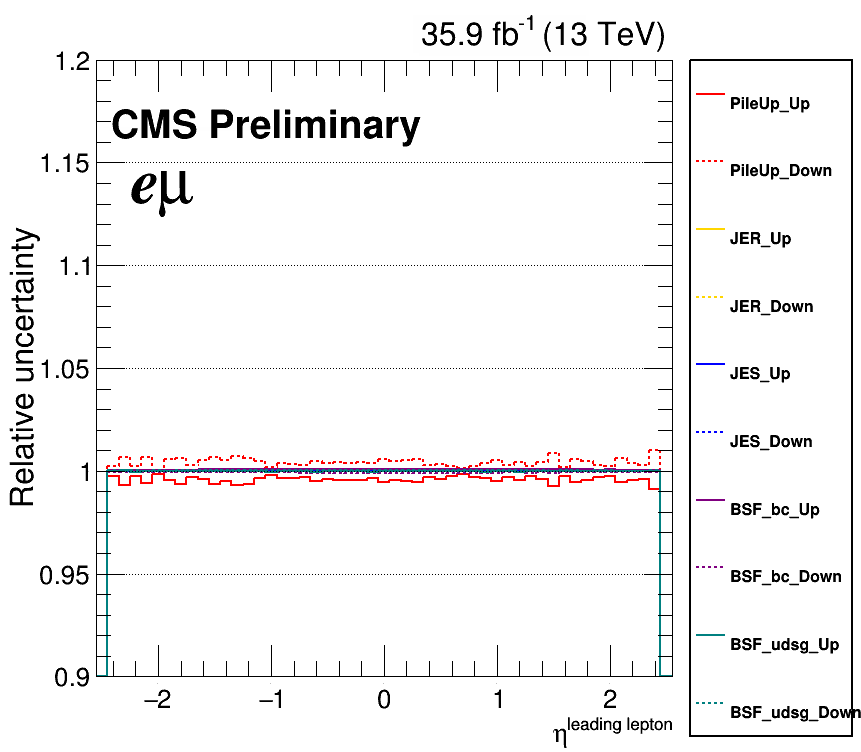
\includegraphics[width=0.32\textwidth]{figures/tW/fig/Step2/emu_shape_uncert/Shape_uncert_H_lepton_led_eta.png}&
%      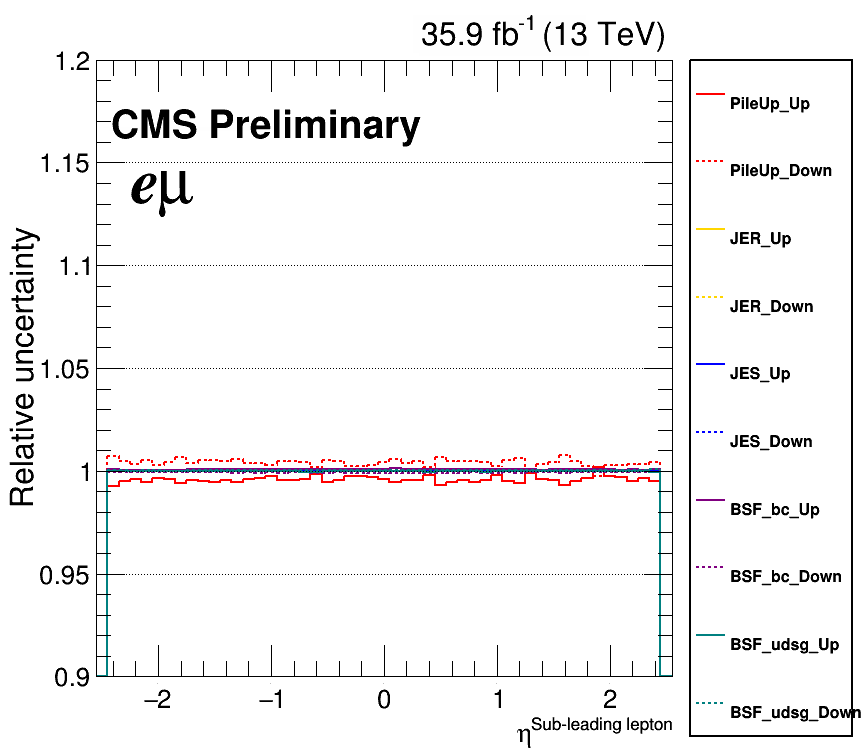
\includegraphics[width=0.32\textwidth]{figures/tW/fig/Step2/emu_shape_uncert/Shape_uncert_H_lepton_sub_eta.png}\\
%      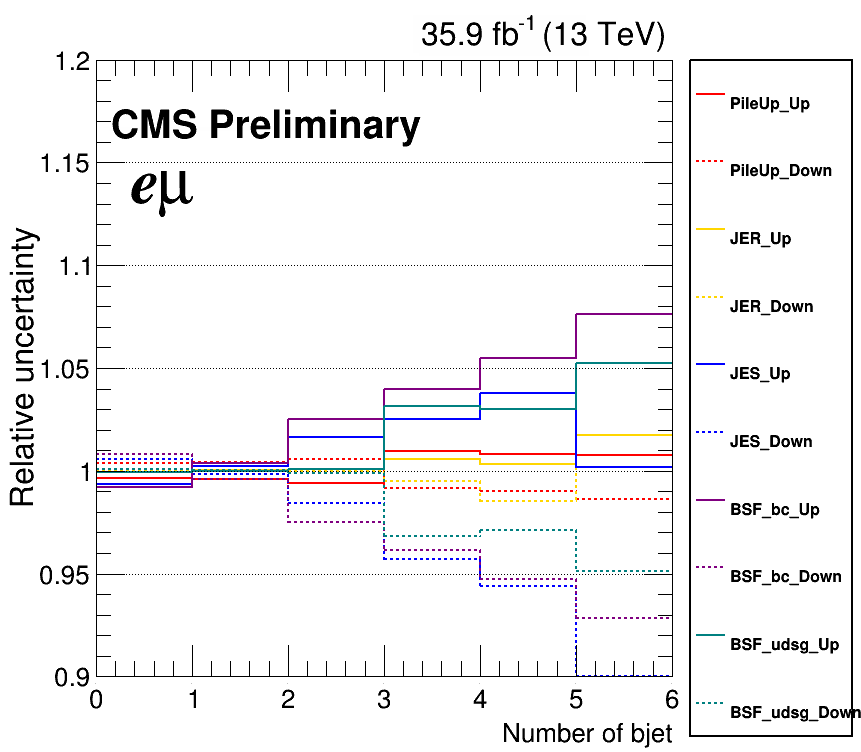
\includegraphics[width=0.32\textwidth]{figures/tW/fig/Step2/emu_shape_uncert/Shape_uncert_H_N_b_jets.png}&
%      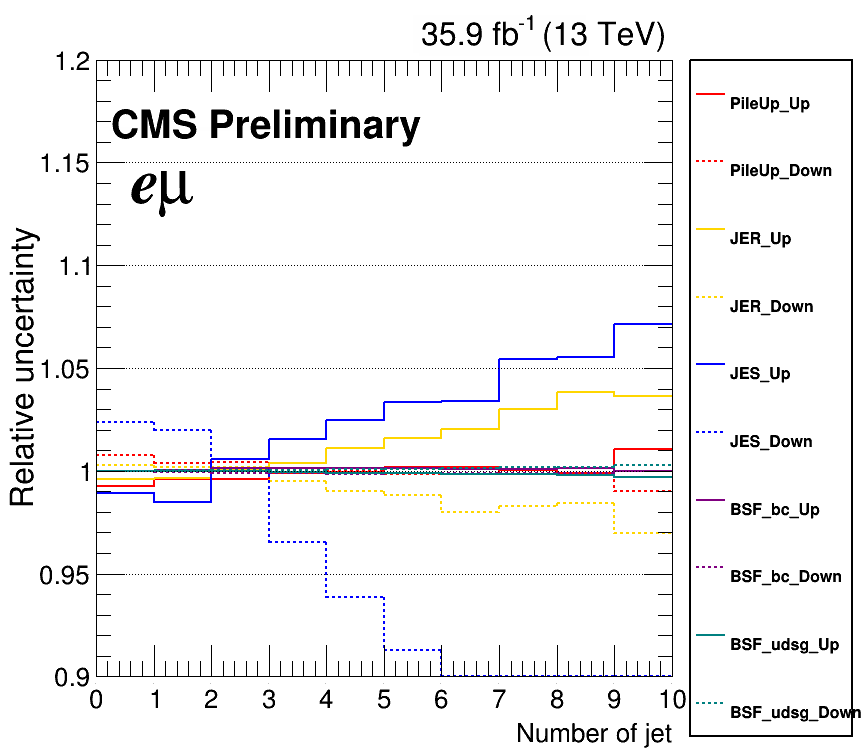
\includegraphics[width=0.32\textwidth]{figures/tW/fig/Step2/emu_shape_uncert/Shape_uncert_H_N_loose_jets.png}\\
%      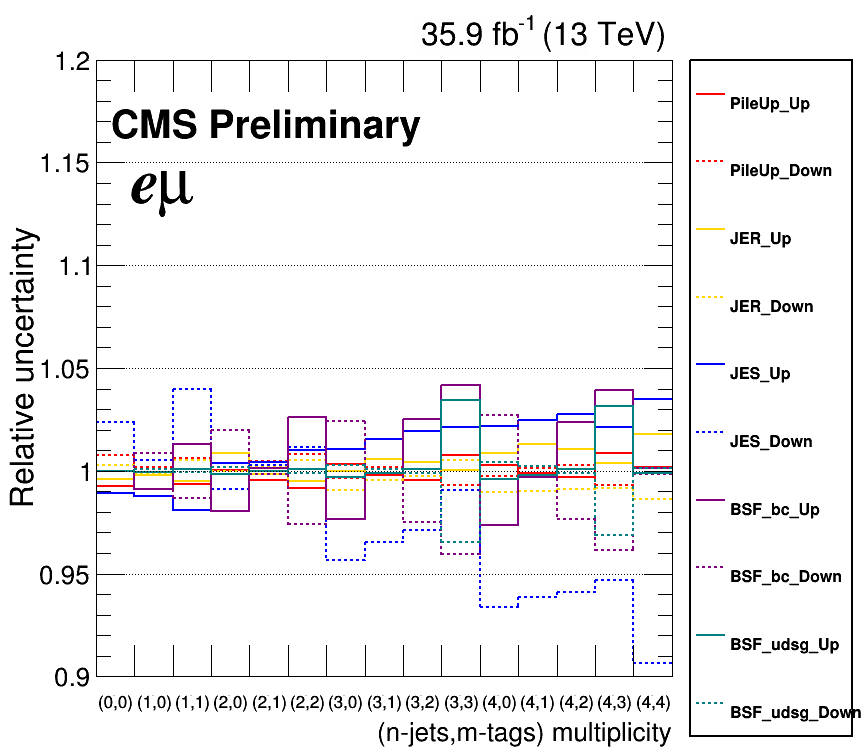
\includegraphics[width=0.32\textwidth]{figures/tW/fig/Step2/emu_shape_uncert/Shape_uncert_H_njet_bjet.png}&
%      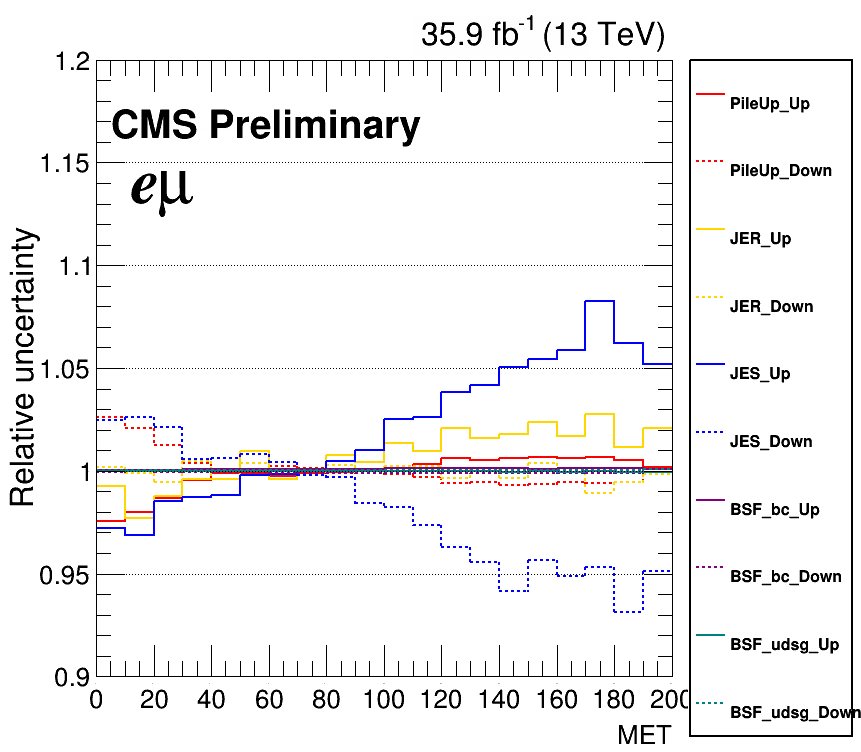
\includegraphics[width=0.32\textwidth]{figures/tW/fig/Step2/emu_shape_uncert/Shape_uncert_H_MET_Et.png}\\
%    \end{tabular}
%    \caption{The distributions of leading (or sub-leading) lepton Pt, $\eta$ and number of jet, number of b jet, number of (jet, bjet) and MET for different shape dependent uncertainty after step 2.
%    \label{fig:shape_uncert}}
%  \end{center}
%\end{figure}
%


\begin{figure}[ht]
  \begin{center}
    \begin{tabular}{ccc}
      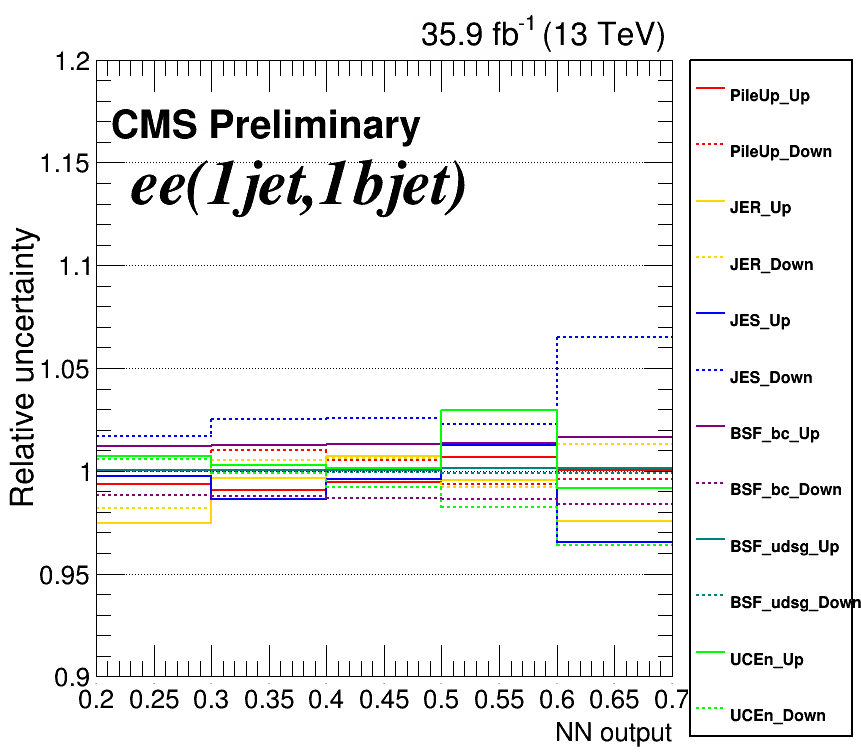
\includegraphics[width=0.4\textwidth]{figures/tW/fig/Step2/uncertainties/ee/Shape_uncert_H_MLP_1jet_1bjet_comb.png} &
      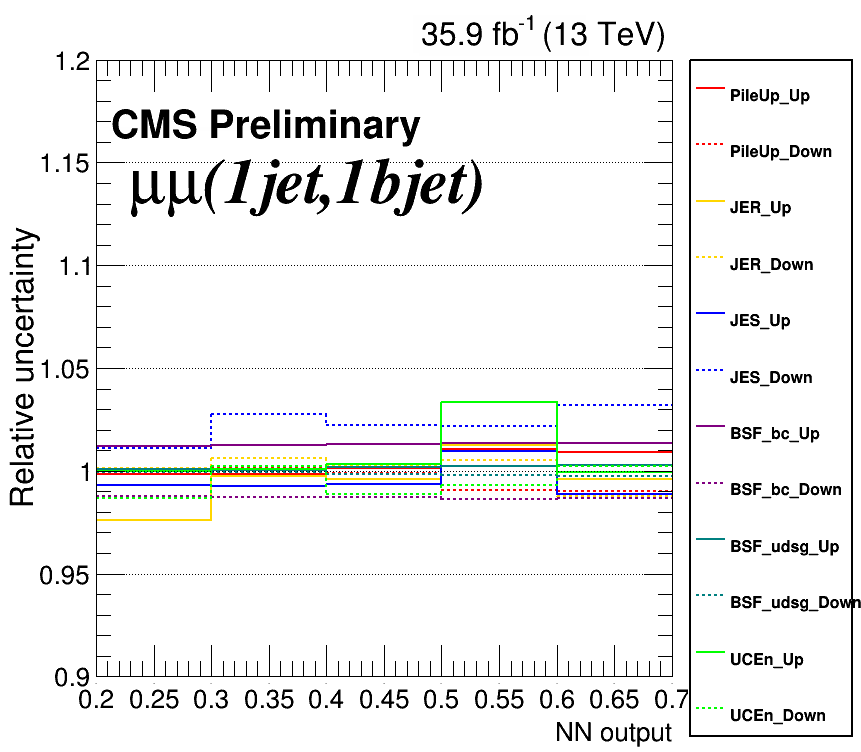
\includegraphics[width=0.4\textwidth]{figures/tW/fig/Step2/uncertainties/mumu/Shape_uncert_H_MLP_1jet_1bjet_comb.png}\\
      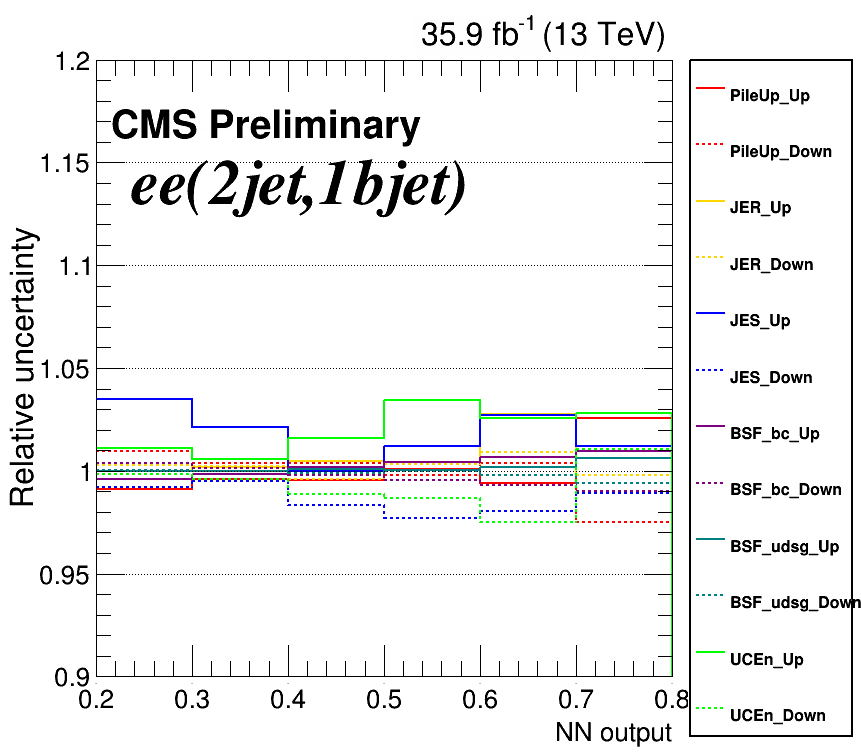
\includegraphics[width=0.4\textwidth]{figures/tW/fig/Step2/uncertainties/ee/Shape_uncert_H_MLP_2jet_1bjet_comb.png} &
      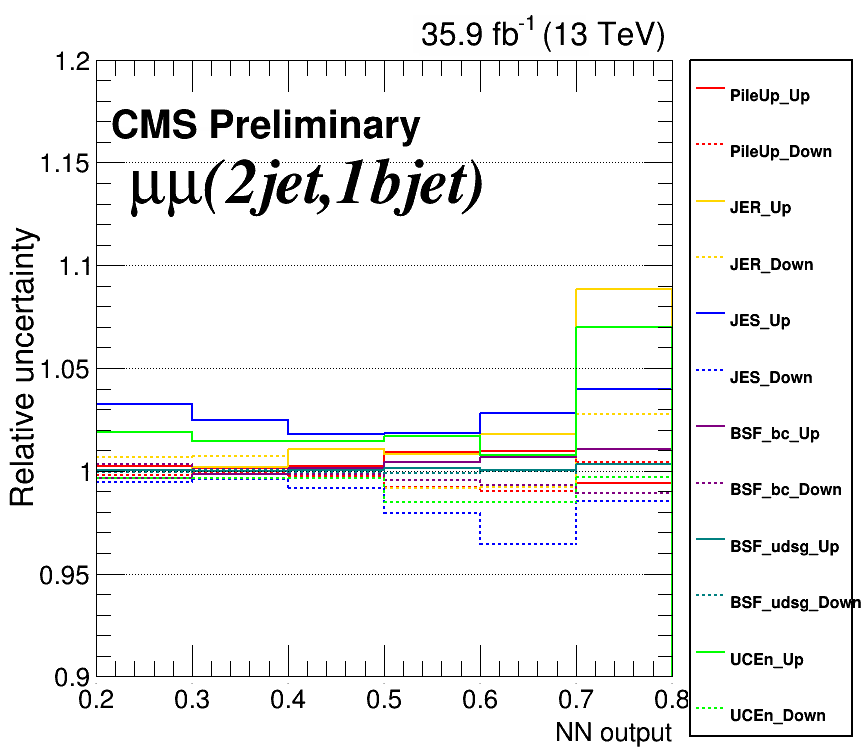
\includegraphics[width=0.4\textwidth]{figures/tW/fig/Step2/uncertainties/mumu/Shape_uncert_H_MLP_2jet_1bjet_comb.png}\\
    \end{tabular}
    \caption{The relative effect of the shape dependent uncertainties in MLP distribution for different (1jet,1b-jet)  region (top row), (2jet,1b-jet) region (bottom row) for $ee$ channel (left column) and $\mu\mu$ channel (right column).
    \label{fig:uncert_shape}}
  \end{center}
\end{figure}


%
\begin{table}[]
\centering
\caption{all systematic uncertainty effect for $e\mu$ channel}
\label{tab:emu_all}
\scalebox{0.8}{
\begin{tabular}{|l|c|c|c|c|c|}
\hline
all                                 & all                                              & 1jet, 0bjet                                       & 1jet, 1bjet                                       & 2jet, 1bjet                                      & $>=2$jet, 2bjet     \\ \hline
nominal                                 & 360368.715                                  & 50038.169                                  & 37673.412                                  & 51381.557                                 & 49390.530             \\ \hline \hline
luminosity\_up                           & 2.373\%                            & 2.297\%                            & 2.451\%                            & 2.457\%                           & 2.471\%                            \\ \hline 
luminosity\_down                         & -2.373\%                          & -2.297\%                          & -2.451\%                          & -2.457\%                         & -2.471\%                          \\ \hline 
TT\_up                  & 3.193\%                   & 2.354\%                   & 4.039\%                   & 4.594\%                  & 4.789\%                   \\ \hline 
TT\_down                & -3.193\%                 & -2.354\%                 & -4.039\%                 & -4.594\%                & -4.789\%                 \\ \hline 
DY\_up  & 2.703\%   & 3.403\%   & 0.744\%   & 0.270\%  & 0.032\%   \\ \hline 
DY\_down& -2.703\% & -3.403\% & -0.744\% & -0.270\%& -0.032\% \\ \hline 
Jets\_up                       & 1.026\%                        & 1.410\%                        & 0.393\%                        & 0.383\%                       & 0.233\%                        \\ \hline 
Jets\_down                     & -1.026\%                      & -1.410\%                      & -0.393\%                      & -0.383\%                     & -0.233\%                      \\ \hline 
other\_up                          & 6.431\%                           & 11.745\%                           & 0.385\%                           & 0.262\%                          & 0.245\%                           \\ \hline 
other\_down                        & -6.431\%                         & -11.745\%                         & -0.385\%                         & -0.262\%                        & -0.245\%                         \\ \hline \hline 
TriggerSF\_up                               & 0.677\%                                & 0.692\%                                & 0.679\%                                & 0.656\%                               & 0.638\%                                \\ \hline 
TriggerSF\_down                             & -0.677\%                              & -0.692\%                              & -0.679\%                              & -0.656\%                             & -0.638\%                              \\ \hline 
PileUp\_up                             & -0.415\%                              & -0.198\%                              & -0.657\%                              & -0.463\%                             & -0.610\%                              \\ \hline 
PileUp\_down                           & 0.408\%                            & 0.191\%                            & 0.642\%                            & 0.451\%                           & 0.588\%                            \\ \hline 
JER\_up                         & -0.001\%                          & -0.200\%                          & -0.515\%                          & -0.180\%                         & 0.092\%                          \\ \hline     
JER\_down                       & -0.002\%                        & -0.117\%                        & 0.536\%                        & 0.168\%                       & -0.010\%                        \\ \hline    
JES\_up                                 & -0.001\%                                  & -1.242\%                                  & -1.886\%                                  & 0.441\%                                 & 1.664\%                                  \\ \hline    
JES\_down                               & -0.005\%                                & 0.524\%                                & 3.970\%                                & 0.260\%                               & -1.567\%                                \\ \hline    
BTagSF\_bc\_up                              & 0.083\%                               & -0.876\%                               & 1.302\%                               & 0.123\%                              & 2.530\%                               \\ \hline    
BTagSF\_bc\_down                            & -0.083\%                             & 0.876\%                             & -1.302\%                             & -0.154\%                            & -2.501\%                             \\ \hline    
BTagSF\_udsg\_up                            & -0.025\%                             & -0.085\%                             & 0.082\%                             & -0.001\%                            & 0.105\%                             \\ \hline     
BTagSF\_udsg\_down                          & 0.025\%                           & 0.085\%                           & -0.082\%                           & 0.001\%                          & -0.105\%                           \\ \hline     
EleRecoSF\_up                            & 0.493\%                             & 0.490\%                             & 0.499\%                             & 0.498\%                            & 0.500\%                             \\ \hline    
EleRecoSF\_down                          & -0.493\%                           & -0.490\%                           & -0.499\%                           & -0.498\%                          & -0.500\%                           \\ \hline    
EleIDIsoSF\_up                              & 1.273\%                               & 1.261\%                               & 1.283\%                               & 1.287\%                              & 1.295\%                               \\ \hline    
EleIDIsoSF\_down                            & -1.273\%                             & -1.261\%                             & -1.283\%                             & -1.287\%                            & -1.295\%                             \\ \hline        
MuIDSF\_up                             & 1.170\%                              & 1.161\%                              & 1.146\%                              & 1.148\%                             & 1.150\%                              \\ \hline    
MuIDSF\_down                           & -1.170\%                            & -1.161\%                            & -1.146\%                            & -1.148\%                           & -1.150\%                            \\ \hline    
MuIsoSF\_up                            & 0.501\%                             & 0.498\%                             & 0.505\%                             & 0.505\%                            & 0.507\%                             \\ \hline           
MuIsoSF\_down                          & -0.501\%                           & -0.498\%                           & -0.505\%                           & -0.505\%                          & -0.507\%                           \\ \hline    
MuTrackSF\_up                          & 0.017\%                           & 0.017\%                           & 0.017\%                           & 0.016\%                          & 0.016\%                           \\ \hline    
MuTrackSF\_down                        & -0.017\%                         & -0.017\%                         & -0.017\%                         & -0.016\%                        & -0.016\%                         \\ \hline \hline 
DY\_PDF\_Up                        & 0.037\%                         & 0.195\%                         & 0.000\%                         & 0.000\%                        & 0.000\%                         \\ \hline    
DY\_PDF\_Down                      & -0.163\%                       & -0.158\%                       & 0.000\%                       & 0.000\%                      & 0.000\%                       \\ \hline    
DY\_QCD\_Up                        & 0.179\%                         & 0.937\%                         & 0.000\%                         & 0.000\%                        & 0.000\%                         \\ \hline    
DY\_QCD\_Down                      & -0.289\%                       & -0.882\%                       & 0.000\%                       & 0.000\%                      & 0.000\%                       \\ \hline    
ISR\_down                              & 0.998\%                                     & 1.563\%                                  & 1.708\%                                  & 2.628\%                                    & 0.593\%                               \\ \hline
ISR\_up                                & 0.152\%                                       & -0.439\%                                    & -0.321\%                                    & -0.567\%                                      & -0.433\%                                 \\ \hline
FSR\_down                              & 1.150\%                                     & -1.409\%                                  & 0.603\%                                  & 1.848\%                                    & 5.822\%                               \\ \hline
FSR\_up                                & -0.313\%                                       & 4.215\%                                    & 0.350\%                                    & -0.368\%                                      & -7.702\%                                 \\ \hline 
TT\_CR\_Up                      & 1.210\%                             & 0.514\%                          & 0.764\%                          & 1.637\%                          & 1.155\%                         \\ \hline        
TT\_CR\_Down                    & 0.230\%                           & -0.089\%                        & -1.417\%                        & 0.019\%                       & 0.166\%                        \\ \hline        
TT\_PDF\_Up                        & 0.260\%                         & 0.122\%                         & 0.367\%                         & 0.451\%                        & 0.546\%                         \\ \hline    
TT\_PDF\_Down                      & -0.350\%                       & -0.168\%                       & -0.399\%                       & -0.621\%                      & -0.685\%                       \\ \hline    
TT\_QCD\_Up                        & 0.149\%                         & 0.341\%                         & 0.883\%                         & 0.679\%                        & 0.370\%                         \\ \hline    
TT\_QCD\_Down                      & -0.267\%                       & -0.529\%                       & -1.233\%                       & -1.114\%                      & -0.515\%                       \\ \hline    
TT\_TopMass\_down                      & 0.022\%                       & 0.284\%                       & 0.355\%                       & -0.100\%                      & -0.429\%                       \\ \hline    
TT\_TopMass\_up                      & 0.263\%                       & -0.014\%                       & -0.147\%                       & 0.433\%                      & 0.580\%                       \\ \hline        
TT\_Tune\_down            & 0.814\%             & 0.628\%             & 0.485\%             & 1.235\%            & 0.447\%             \\ \hline      
TT\_Tune\_up              & 0.487\%               & 0.298\%               & 0.413\%               & 0.662\%              & -0.061\%               \\ \hline    
TT\_hdamp\_down                  & 0.973\%                         & 1.358\%                      & 3.327\%                      & 2.112\%                        & 1.024\%                   \\ \hline
TT\_hdamp\_up                    & 0.672\%                           & 0.321\%                        & -0.997\%                        & 0.335\%                          & 0.372\%                     \\ \hline
TW\_DS                      & -0.088\%                             & 0.317\%                          & 0.832\%                          & -0.394\%                            & -0.514\%                       \\ \hline
TW\_TopMass\_down                & -0.006\%                       & 0.011\%                    & -0.051\%                    & -0.026\%                      & -0.011\%                 \\ \hline
TW\_TopMass\_up                & 0.006\%                       & 0.016\%                    & 0.010\%                    & 0.006\%                      & 0.012\%                 \\ \hline
TW\_MEscale\_down             & -0.017\%                    & -0.049\%                 & -0.479\%                 & -0.009\%                   & 0.125\%              \\ \hline
TW\_MEscale\_up               & 0.017\%                      & 0.284\%                   & 0.459\%                   & -0.202\%                     & -0.120\%                \\ \hline
total\_up                          & 8.719\%                           & 13.839\%                           & 7.917\%                           & 7.228\%                          & 8.966\%                           \\ \hline 
total\_down                        & -8.372\%                         & -13.113\%                         & -6.172\%                         & -5.822\%                        & -10.143\%                         \\ \hline \hline 
\end{tabular}}
\end{table}


\begin{table}[]
\centering
\caption{all systematic uncertainty effect for ee channel}
\label{tab:ee_all}
\scalebox{0.8}{
\begin{tabular}{|l|c|c|c|c|}
\hline
all                                 & all                                              & 1jet, 1bjet                                       & 2jet, 1bjet                                      & $>=2$jet, 2bjet     \\ \hline
nominal                                 & 64928.258                                  & 5936.414                                  & 8330.690                                 & 7973.390             \\ \hline \hline
luminosity\_up                           & 2.438\%                            & 2.480\%                            & 2.459\%                           & 2.459\%                            \\ \hline 
luminosity\_down                         & -2.436\%                          & -2.453\%                          & -2.459\%                         & -2.459\%                          \\ \hline 
TT\_up                  & 2.877\%                   & 3.993\%                   & 4.489\%                  & 4.742\%                   \\ \hline 
TT\_down                & -2.877\%                 & -3.993\%                 & -4.489\%                & -4.742\%                 \\ \hline 
DY\_up  & 8.886\%   & 1.305\%   & 0.867\%  & 0.173\%   \\ \hline 
DY\_down& -8.886\% & -1.305\% & -0.867\%& -0.173\% \\ \hline 
Jets\_up                       & 0.393\%                        & 0.010\%                        & 0.105\%                       & 0.136\%                        \\ \hline 
Jets\_down                     & -0.393\%                      & -0.010\%                      & -0.105\%                     & -0.136\%                      \\ \hline 
other\_up                          & 3.730\%                           & 0.287\%                           & 0.290\%                          & 0.313\%                           \\ \hline 
other\_down                        & -3.730\%                         & -0.287\%                         & -0.290\%                        & -0.313\%                         \\ \hline \hline 
TriggerSF\_up                               & 0.834\%                                & 0.829\%                                & 0.809\%                               & 0.792\%                                \\ \hline 
TriggerSF\_down                             & -0.834\%                              & -0.829\%                              & -0.809\%                             & -0.792\%                              \\ \hline 
PileUp\_up                             & 2.883\%                              & -0.035\%                              & -0.220\%                             & -0.630\%                              \\ \hline 
PileUp\_down                           & -2.757\%                            & 0.026\%                            & 0.162\%                           & 0.616\%                            \\ \hline 
JER\_up                         & 6.354\%                          & -0.022\%                          & 0.520\%                         & 0.736\%                          \\ \hline     
JER\_down                       & 1.454\%                        & -0.055\%                        & -0.229\%                       & -0.024\%                        \\ \hline    
JES\_up                                 & 5.257\%                                  & 0.215\%                                  & 1.167\%                                 & 3.161\%                                  \\ \hline    
JES\_down                               & -4.670\%                                & 2.485\%                                & -1.465\%                               & -2.931\%                                \\ \hline    
BTagSF\_bc\_up                              & 0.073\%                               & 1.333\%                               & 0.207\%                              & 2.520\%                               \\ \hline    
BTagSF\_bc\_down                            & -0.073\%                             & -1.333\%                             & -0.236\%                            & -2.491\%                             \\ \hline    
BTagSF\_udsg\_up                            & -0.022\%                             & 0.082\%                             & 0.081\%                            & 0.127\%                             \\ \hline     
BTagSF\_udsg\_down                          & 0.022\%                           & -0.082\%                           & -0.081\%                          & -0.128\%                           \\ \hline     
EleRecoSF\_up                            & 1.002\%                             & 1.009\%                             & 1.006\%                            & 1.004\%                             \\ \hline    
EleRecoSF\_down                          & -0.997\%                           & -1.004\%                           & -1.001\%                          & -0.999\%                           \\ \hline    
EleIDIsoSF\_up                              & 2.601\%                               & 2.618\%                               & 2.623\%                              & 2.620\%                               \\ \hline    
EleIDIsoSF\_down                            & -2.568\%                             & -2.584\%                             & -2.589\%                            & -2.586\%                             \\ \hline        
UnclusteredEn\_up                         & 10.246\%                          & 1.408\%                          & 1.779\%                         & 0.896\%                          \\ \hline    
UnclusteredEn\_down                      & -3.109\%                         & -1.304\%                        & -0.891\%                       & -0.534\%                        \\ \hline   \hline 
ISR\_down                                & 0.596\%                                   & 1.777\%                                  & 1.501\%                                 & -0.052\%                                  \\ \hline
ISR\_up                                  & -0.217\%                                     & -1.427\%                                    & -1.480\%                                   & -0.689\%                                    \\ \hline
FSR\_down                                & 0.862\%                                   & 0.779\%                                  & 1.462\%                                 & 6.013\%                                  \\ \hline
FSR\_up                                  & -0.832\%                                     & -1.802\%                                    & -1.003\%                                   & -7.126\%                                    \\ \hline 
TT\_CR\_Up                        & 1.435\%                           & -0.552\%                          & 0.502\%                         & 1.733\%                          \\ \hline        
TT\_CR\_Down                      & -0.475\%                         & -1.515\%                        & -0.235\%                       & 0.418\%                        \\ \hline        
TT\_PDF\_Up                        & 0.203\%                         & 0.007\%                         & 0.556\%                        & 0.602\%                       \\ \hline    
TT\_PDF\_Down                      & -0.306\%                       & -0.668\%                       & -0.401\%                      & -0.553\%                       \\ \hline    
TT\_QCD\_Up                        & 0.076\%                         & 0.631\%                         & 0.740\%                        & 0.315\%                       \\ \hline    
TT\_QCD\_Down                      & -0.164\%                       & -1.691\%                       & -0.833\%                      & -0.271\%                       \\ \hline    
TT\_TopMass\_down                      & -0.106\%                       & 0.161\%                       & -0.172\%                      & -0.752\%                       \\ \hline    
TT\_TopMass\_up                      & 0.313\%                       & 0.168\%                       & 0.669\%                      & 0.746\%                       \\ \hline        
TT\_Tune\_down            & 0.544\%             & 1.322\%             & 0.711\%            & 0.320\%             \\ \hline      
TT\_Tune\_up              & 0.252\%               & 1.386\%               & -0.059\%              & 0.446\%               \\ \hline    
TT\_hdamp\_down                  & 0.105\%                         & 3.320\%                      & 1.957\%                        & 0.024\%                   \\ \hline
TT\_hdamp\_up                    & 0.789\%                           & -0.098\%                        & 0.269\%                          & 1.191\%                     \\ \hline
TW\_DS                      & -0.287\%                             & 0.699\%                          & -0.656\%                            & -0.776\%                       \\ \hline
TW\_TopMass\_down                & -0.025\%                       & -0.080\%                    & -0.026\%                      & -0.035\%                 \\ \hline
TW\_TopMass\_up                & 0.024\%                       & 0.064\%                    & 0.008\%                      & 0.056\%                 \\ \hline
TW\_MEscale\_down             & -0.021\%                    & -0.764\%                 & 0.212\%                   & 0.275\%              \\ \hline
TW\_MEscale\_up               & -0.118\%                      & 0.169\%                   & -0.129\%                     & -0.307\%                \\ \hline
total\_up                          & 17.429\%                           & 7.865\%                           & 7.131\%                          & 9.870\%                           \\ \hline 
total\_down                        & -12.504\%                         & -6.885\%                         & -6.564\%                        & -10.266\%                         \\ \hline \hline 
\end{tabular}}
\end{table}


\begin{table}[]
\centering
\caption{all systematic uncertainty effect for $\mu\mu$ channel}
\label{tab:mumu_all}
\scalebox{0.8}{
\begin{tabular}{|l|c|c|c|c|}
\hline
all                                 & all                                              & 1jet, 1bjet                                       & 2jet, 1bjet                                      & $>=2$jet, 2bjet     \\ \hline
nominal                                 & 138879.681                                  & 12365.806                                  & 16751.491                                 & 15888.515             \\ \hline \hline
luminosity\_up                           & 2.457\%                            & 2.469\%                            & 2.469\%                           & 2.490\%                            \\ \hline 
luminosity\_down                         & -2.457\%                          & -2.469\%                          & -2.469\%                         & -2.490\%                          \\ \hline 
TT\_up                  & 2.688\%                   & 3.922\%                   & 4.473\%                  & 4.763\%                   \\ \hline 
TT\_down                & -2.688\%                 & -3.922\%                 & -4.473\%                & -4.763\%                 \\ \hline 
DY\_up  & 10.341\%   & 1.806\%   & 0.896\%  & 0.154\%   \\ \hline 
DY\_down& -10.341\% & -1.806\% & -0.896\%& -0.154\% \\ \hline 
Jets\_up                       & 0.483\%                        & 0.351\%                        & 0.399\%                       & 0.101\%                        \\ \hline 
Jets\_down                     & -0.483\%                      & -0.351\%                      & -0.399\%                     & -0.101\%                      \\ \hline 
other\_up                          & 3.655\%                           & 0.330\%                           & 0.291\%                          & 0.261\%                           \\ \hline 
other\_down                        & -3.655\%                         & -0.330\%                         & -0.291\%                        & -0.261\%                         \\ \hline \hline 
TriggerSF\_up                               & 0.639\%                                & 0.663\%                                & 0.650\%                               & 0.643\%                                \\ \hline 
TriggerSF\_down                             & -0.639\%                              & -0.663\%                              & -0.650\%                             & -0.643\%                              \\ \hline 
PileUp\_up                             & 3.973\%                              & 0.568\%                              & 0.372\%                             & 0.038\%                              \\ \hline 
PileUp\_down                           & -3.749\%                            & -0.484\%                            & -0.364\%                           & -0.045\%                            \\ \hline 
JER\_up                         & 6.743\%                          & 0.354\%                          & 1.174\%                         & 0.769\%                          \\ \hline     
JER\_down                       & 2.153\%                        & 0.367\%                        & 0.051\%                       & -0.012\%                        \\ \hline    
JES\_up                                 & 6.038\%                                  & -0.217\%                                  & 2.174\%                                 & 3.160\%                                  \\ \hline    
JES\_down                               & -4.781\%                                & 2.199\%                                & -1.209\%                               & -2.834\%                                \\ \hline    
BTagSF\_bc\_up                              & 0.072\%                               & 1.316\%                               & 0.201\%                              & 2.535\%                               \\ \hline    
BTagSF\_bc\_down                            & -0.072\%                             & -1.316\%                             & -0.230\%                            & -2.506\%                             \\ \hline    
BTagSF\_udsg\_up                            & -0.019\%                             & 0.191\%                             & 0.064\%                            & 0.141\%                             \\ \hline     
BTagSF\_udsg\_down                          & 0.019\%                           & -0.191\%                           & -0.064\%                          & -0.140\%                           \\ \hline     
MuIDSF\_up                             & 2.378\%                              & 2.316\%                              & 2.316\%                             & 2.331\%                              \\ \hline    
MuIDSF\_down                           & -2.350\%                            & -2.289\%                            & -2.290\%                           & -2.304\%                            \\ \hline    
MuIsoSF\_up                            & 1.015\%                             & 1.015\%                             & 1.014\%                            & 1.020\%                             \\ \hline           
MuIsoSF\_down                          & -1.010\%                           & -1.010\%                           & -1.009\%                          & -1.015\%                           \\ \hline    
MuTrackSF\_up                          & 0.035\%                           & 0.034\%                           & 0.033\%                          & 0.031\%                           \\ \hline    
MuTrackSF\_down                        & -0.035\%                         & -0.034\%                         & -0.033\%                        & -0.031\%                         \\ \hline  
UnclusteredEn\_up                         & 11.621\%                          & 1.484\%                          & 1.730\%                         & 1.095\%                          \\ \hline    
UnclusteredEn\_down                      & -3.669\%                         & -0.959\%                        & -0.694\%                       & -0.315\%                        \\ \hline   \hline 
ISR\_down                                & 0.663\%                                   & 0.720\%                                  & 2.338\%                                 & -0.018\%                                  \\ \hline
ISR\_up                                  & -0.121\%                                     & -1.984\%                                    & -1.059\%                                   & -0.906\%                                    \\ \hline
FSR\_down                                & 1.006\%                                   & -0.185\%                                  & 1.897\%                                 & 6.035\%                                  \\ \hline
FSR\_up                                  & -0.433\%                                     & 0.220\%                                    & -0.286\%                                   & -7.915\%                                    \\ \hline 
TT\_CR\_Up                         & 1.409\%                          & 0.843\%                          & 0.866\%                         & 1.612\%                           \\ \hline        
TT\_CR\_Down                       & -0.229\%                        & -1.486\%                        & -0.298\%                       & 0.702\%                           \\ \hline        
TT\_PDF\_Up                        & 0.169\%                         & 0.073\%                         & 0.320\%                        & 0.548\%                       \\ \hline    
TT\_PDF\_Down                      & -0.275\%                       & -0.526\%                       & -0.591\%                      & -0.541\%                       \\ \hline    
TT\_QCD\_Up                        & 0.006\%                         & 0.554\%                         & 0.487\%                        & 0.166\%                       \\ \hline    
TT\_QCD\_Down                      & -0.098\%                       & -1.349\%                       & -0.961\%                      & -0.139\%                       \\ \hline    
TT\_TopMass\_down                      & -0.058\%                       & 0.205\%                       & -0.378\%                      & -0.454\%                       \\ \hline    
TT\_TopMass\_up                      & 0.248\%                       & -0.226\%                       & 0.382\%                      & 0.989\%                       \\ \hline        
TT\_Tune\_down            & 0.517\%             & -1.182\%             & 0.669\%            & 1.669\%             \\ \hline      
TT\_Tune\_up              & 0.337\%               & 0.247\%               & 1.175\%              & -1.057\%               \\ \hline    
TT\_hdamp\_down                  & 0.307\%                         & 2.577\%                      & 1.558\%                        & -0.604\%                   \\ \hline
TT\_hdamp\_up                    & 0.279\%                           & -1.488\%                        & -0.518\%                          & -0.526\%                     \\ \hline
TW\_DS                      & -0.193\%                             & 0.629\%                          & -0.636\%                            & -0.596\%                       \\ \hline
TW\_TopMass\_down                & -0.009\%                       & -0.047\%                    & -0.043\%                      & -0.004\%                 \\ \hline
TW\_TopMass\_up                & 0.012\%                       & 0.009\%                    & 0.028\%                      & -0.003\%                 \\ \hline
TW\_MEscale\_down             & 0.042\%                    & -0.349\%                 & 0.026\%                   & 0.160\%              \\ \hline
TW\_MEscale\_up               & -0.063\%                      & -0.134\%                   & -0.161\%                     & -0.068\%                \\ \hline
total\_up                          & 19.567\%                           & 7.066\%                           & 7.604\%                          & 9.886\%                           \\ \hline 
total\_down                        & -13.846\%                         & -6.835\%                         & -6.275\%                        & -10.783\%                         \\ \hline \hline 
\end{tabular}}
\end{table}





